\documentclass{article}
\usepackage[utf8]{inputenc}
\usepackage{geometry}
\geometry{margin=1in}

\usepackage{graphicx}
\graphicspath{{./images/}}

\usepackage{enumerate}
\usepackage{amssymb}
\usepackage{amsmath}
\usepackage{amsthm}

\begin{document}
\newcommand{\R}{\mathbb{R}}
\newcommand{\claim}{\par\noindent\textit{Claim:}\space}

\setcounter{section}{3}
\section{Continuity}

\begin{enumerate}
\setcounter{enumi}{5}
\item If $f$ is defined on $E$, the \textit{graph} of $f$ is the set of points
      $(x, f(x))$ for $x \in E$ or $E \times f(E)$. In particular, if
      $E \subset \R$ and $f: E \to \R$, then the graph of $f$ is a subset of
      the plane ($\R^2$)

Suppose $E$ is compact. Prove that $f$ is continuous on $E$ if and only if its
graph is compact.

\begin{proof}
Let's first suppose that $f$ is not continuous so there's some $p \in E$ where
$\lim_{x\to p} f(x) \neq f(p)$.

Let $\{p_n\} \to p$ be some sequence of $E$ so that
$\{ f(p_n) \} \to y \in \overline{f(E)}$ where $y \neq f(p)$. Then
$\{ (p_n, f(p_n)) \}$ is an infinite subset of the graph of $f$ which has no
limit point in the graph. This must mean the graph is not compact.

Now suppose that $f$ is continuous. Since $E$ is compact then $f(E)$ is
also compact, and it's trivial to show the cartesian product of two compact sets
is also compact.

\end{proof}

\item If $E \subset X$ and if $f$ is a function defined on $X$, the
      \textit{restriction} of $f$ to $E$ is the function $g$ whose domain of
      definition is $E$, such that $g(p) = f(p)$ for $p \in E$.

Define $f,g : \R^2 \to \R$ as

\[
f(x) =
\begin{cases}
                   0 & (x, y) = (0, 0) \\
\frac{xy^2}{x^2+y^4} & (x, y) \neq (0, 0)
\end{cases},\quad
g(x) =
\begin{cases}
                   0 & (x, y) = (0, 0) \\
\frac{xy^2}{x^2+y^6} & (x, y) \neq (0, 0)
\end{cases}
\]

and prove the following:
\begin{enumerate}[a.]
\item $f$ is bounded on $\R^2$
\item $g$ is unbounded in every neighborhood of $(0, 0)$
\item $f$ is not continuous at $(0, 0)$
\item The restriction of both $f$ and $g$ to any line in $\R^2$ is continuous
\end{enumerate}

\qquad

\begin{enumerate}[a.]
\newcommand{\Boundary}{\frac{1}{2}}

\item \claim $f(x, y) \in [-\Boundary, \Boundary]$
      for $(x, y) \in \R^2$.
\begin{proof}
We can equivalently say that $f(x,y) \leq \Boundary$ if $x^2 + y^4 \geq 2xy^2$.
If we plot the functions on either side of the inequality, we can visualize
that the inequality is true ($x^2 + y^4$ is pictured here in orange).

\begin{figure}[h]
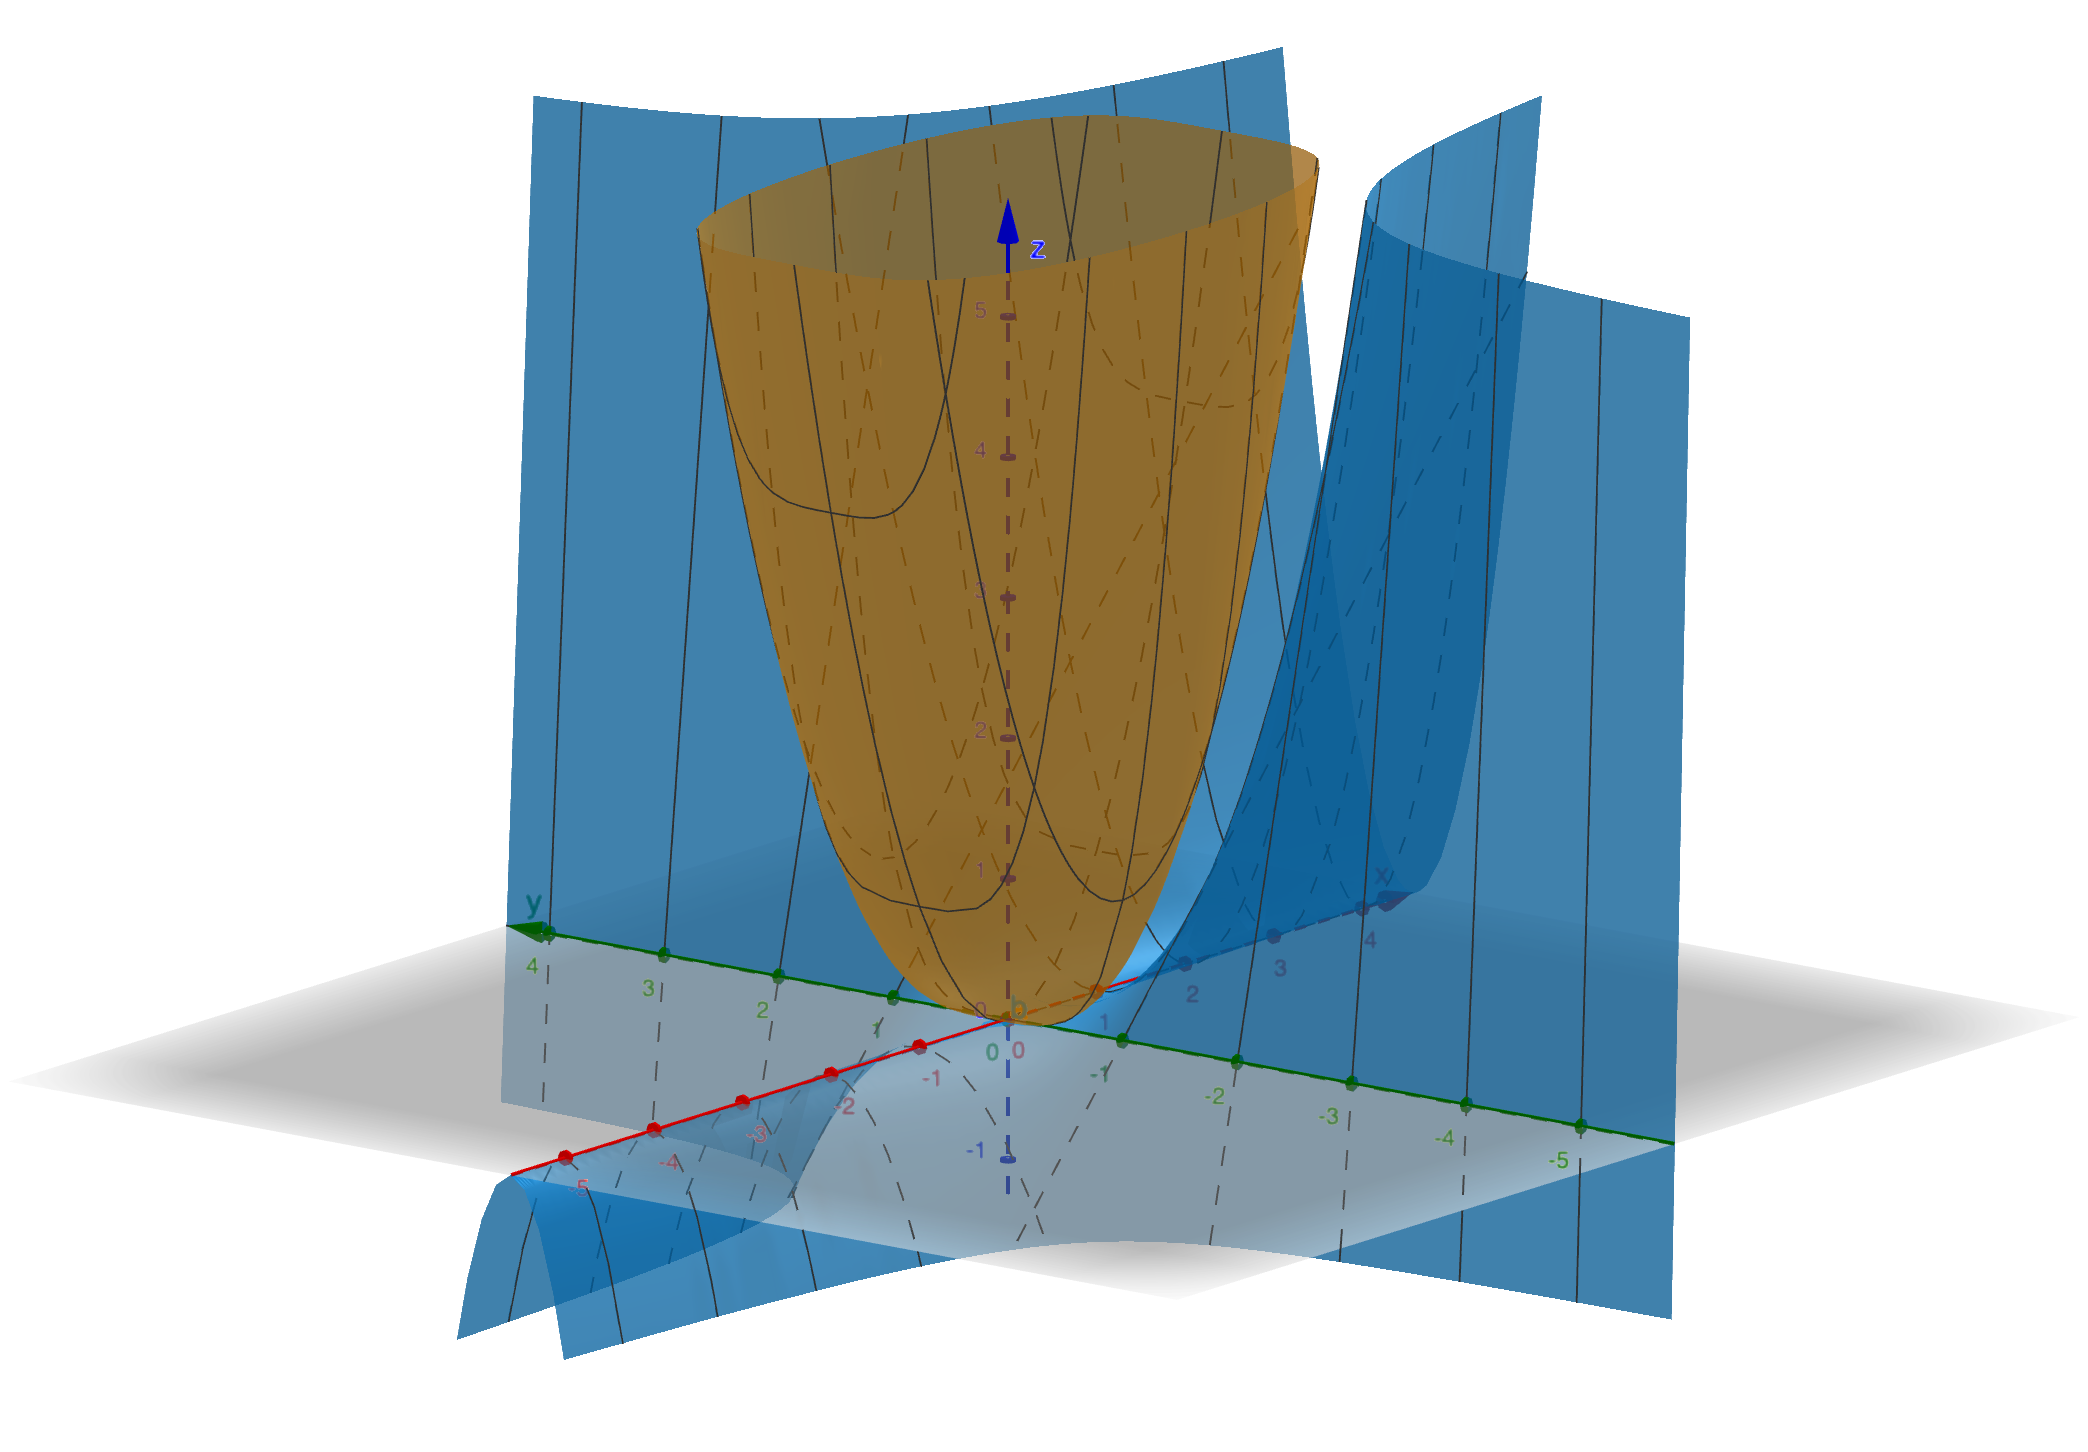
\includegraphics[scale=0.1]{figure-04-07-a}
\centering
\end{figure}

To show this rigorously, let's rearrange the inequality to a quadratic form with
respect to $y^2$:
\begin{equation*}
\begin{split}
y^4 - 2xy^2 + x^2 &\geq 0 \\
      (y^2 - x)^2 &\geq 0
\end{split}
\end{equation*}
This is clearly true for all $(x, y) \in \R^2$. We can similarly show that
$f(x, y) \geq -\Boundary$ with the statement $(y^2 + x)^2 \geq 0$. This tells
us that $f$ is bounded.

\end{proof}

\end{enumerate}
        
\end{enumerate}

\end{document}
